\chapter{Work Plan}
\begin{figure}
    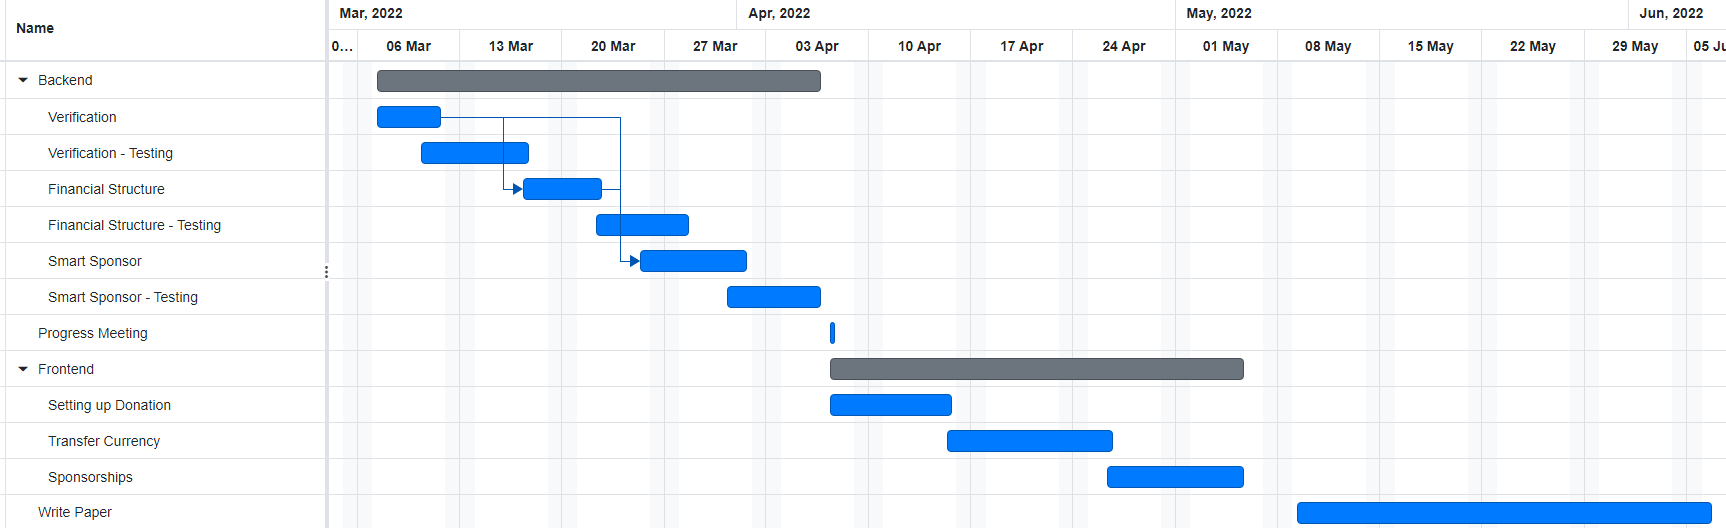
\includegraphics[width=1 \textwidth]{figures/timeplan.PNG}  
    \caption{Project plan for this Bachelor Thesis}
    \label{fig:my_label}
\end{figure}
Assuming 12 weeks are available for this project the work plan is structured into 3 parts, as seen in Fig 4.1.\\
The first 4 weeks are allocated to programming the backend. As this is a blockchain-based application this means everything to do with Ethereum. Using truffle the 3 backend systems detailed in chapter 3 will be tested to ensure correct code.\\
After the backend development, a meeting regarding general progress will be held with the supervisor.\\
The next 4 weeks will be used on the frontend development. Both the general JavaScript for the backend and the connection to Metamask are aspects that will require research. CSS will be done via bootstrap.\\
In the final 4 weeks, the paper will be written. This step is more flexible as parts of this could be done during the 8 preceding weeks. The final presentation will also be created during this time.